\documentclass[11pt]{article}

\usepackage{setspace}
\usepackage[margin=1in]{geometry}

% Make table of contents look better
\usepackage{tabularx}
\usepackage{tocloft}
\renewcommand{\cftsecleader}{\cftdotfill{\cftdotsep}}

\usepackage{graphicx}
\usepackage{pdfpages}
\usepackage{hyperref}

% \usepackage[ngerman]{babel}
% \usepackage[T1]{fontenc}
% \usepackage[ansinew]{inputenc}
% \usepackage{lmodern}

% Times New Roman font
\usepackage{txfonts}

\begin{document}

\setlength{\parindent}{2em}

\begin{titlepage}
\clearpage
\thispagestyle{empty}

\begin{center}
{\bf Technical Communication for Computer Scientists: 15-221}\\
{\bf Spring 2015}\\

\vspace{25 mm}

{\bf Progress Report:}\\
{\bf C0 Debugger}\\
\vspace{25 mm}

Aaron Gutierrez\\
Mitchell Plamann\\
Shyam Raghavan\\
Suhaas Reddy\\

\vspace{25 mm}

{\bf Submitted to}\\
Thomas M. Keating\\
Assistant Teaching Professor\\
Computer Science Department\\
School of Computer Science\\

\vspace{25 mm}

{\bf Prepared and Submitted by}\\
Shyam Raghavan - April 14, 2015
\end{center}
\end{titlepage}

\pagenumbering{roman}
\tableofcontents
\newpage

\pagenumbering{arabic}

\section{Overview}
\subsection{Purpose of the Report}
This report serves as an update to the reader on the progress the c0db team has
made on the C0 Debugger during the first month of work. The report will detail
what has been accomplished so far, what is in progress, what is planned for the
future, and any changes that will be made to the original plan of action. In
addition, the report will detail new literature that has been gathered and
used.
\subsection{Purpose of the Project}
The purpose of this project is to build a web application that can debug C0
code and can aid in a student's understanding of fundamental computational
models. This project will benefit students in 15-122 Principals of Imperative
Computation at Carnegie Mellon University by helping them create correct
programs. The C0 Debugger will enable students to understand how their programs
execute and find where problems originate more easily than with existing tools.
In addition to debugging, students will have better knowledge for how the
underlying computation model works when evaluating their code.
\par
The C0 Debugger will also enable students to test simple programs with little
setup, using only a web browser. They will no longer have to set up and become
familiar with a Unix environment before they can program, making C0 accessible
to more people, more quickly.
\section{Literature Review}
Since the start of our project, we have found multiple new information sources;
the following are the most important ones.
\begin{itemize}
\item Nodeunit documentation \\
    https://github.com/caolan/nodeunit
    \par
    We are using nodeunit to test our virtual machine.
    Since the c0 bytecode has many different opcodes that it uses, it is very
    easy for mistakes in the virtual machine to go unnoticed.
    To prevent this, we are using the nodeunit library to write unit tests for
    our code.
    This has already helped us to find and solve multiple bugs in the VM, and
    having these unit tests will make sure that we can solve any bugs that
    occur as the result of future changes in the code.
\item c0vm Assignment Handout \\
    https://www.cs.cmu.edu/~rjsimmon/15122-f14/prog/c0vm-writeup.pdf
    \par
    This document details how each opcode in the c0 bytecode language works,
    as well as other important implementation details for the c0 virtual
    machine. It has been an important reference while developing a JavaScript
    version of the c0 virtual machine.
\item Common Gateway Interface Support Documentation \\
    https://docs.python.org/2/library/cgi.html
    \par
    This document explains the support module defined by Python 2.7.10 for
    common gateway interfaces. A common gateway interface script is usually
    invoked by a server to process user input submitted through an HTML
    element. This piece of documentation is an important reference for
    developing the flow of information from c0 code to c0 bytecode to a
    working virtual machine.
\end{itemize}
So far, the most important thing we have learned is that good unit tests are
vital for developing this sort of project. Without unit tests that verify
each opcode used by the virtual machine, many bugs would have gone unnoticed,
causing problems later down the line. If we only found these bugs by using
the frontend, they would have been much harder to debug, as there would have
been much more code to work through.
\section{Progress}
\begin{figure}[h]
  \centering
  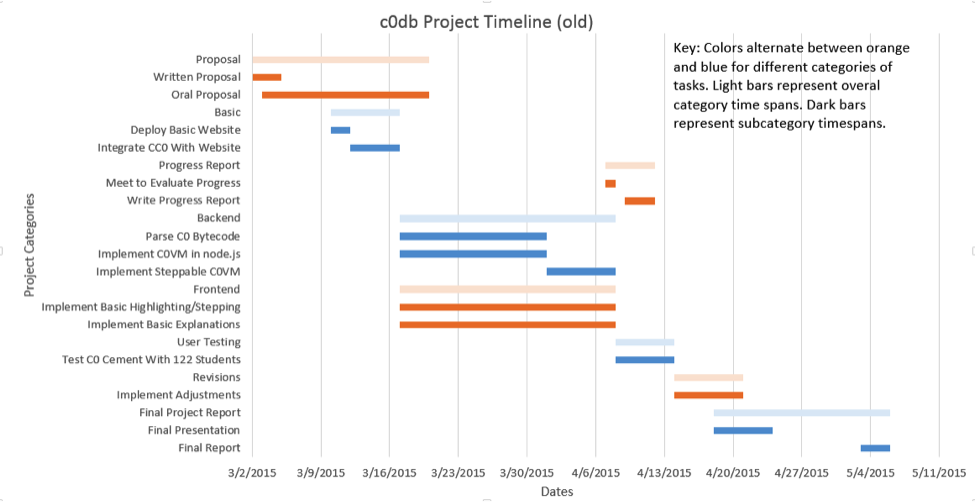
\includegraphics[width=\linewidth]{old-gantt.png}
  \caption{Old Project Gantt Chart}
  \label{fig:old-gantt}
\end{figure}
We are nearing completion on the virtual machine upon which the debugger will
run. Moving forward, the front end team will polish the existing interface, and
expand it to control the debugger. The back end team will work on the core
functionality of the debugger and continue to fix bugs with the virtual machine.
This places us two weeks behind schedule over all, as we planned to have the
virtual machine finished by April 1\textsuperscript{st}.
\subsection{Front End: Status}
The front end team is keeping pace with the back end team, but is still two
weeks behind schedule. We have a working interface where users can input,
compile, and run C0 programs, but there are no debugging features.
\subsection{Front End: Projections}
We will modify our schedule to allow more time for the work on the debugger.
This time will come from a shortened user testing and revision period. That
said, because of our thorough work on the virtual machine, implementing the
debugger should progress more rapidly than originally planned. The modified
schedule is depicted in our updated Gannt chart (Figure 2, below).
\subsection{Back End: Status}
The back end team is also two weeks behind schedule. The virtual machine, along
with most library functions needed to run programs, is complete and working
well. The team has started working on stepping through program execution, but
those features have not yet been incorporated with the rest of the application.
\subsection{Back End: Projections}
In the coming time, the back end team will implement the remaining library
functions, then transition all of their efforts to the debugging features. Like
the front end team, this transition was originally scheduled for
April\textsuperscript{st}, but will now occur in the next week.
\par
\begin{figure}[h]
  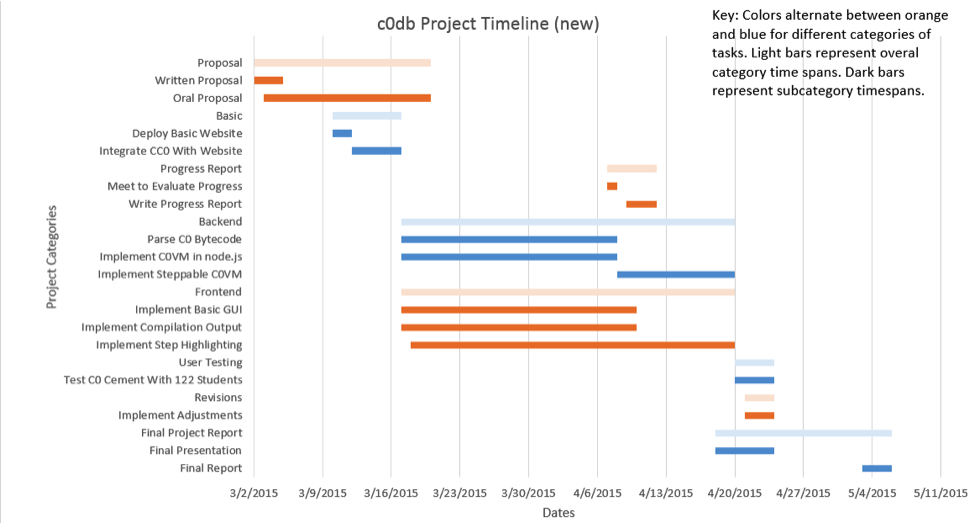
\includegraphics[width=\linewidth]{new-gantt.png}
  \caption{New Project Gantt Chart}
  \label{fig:new-gantt}
\end{figure}
Our revised Gannt chart features two key changes. The back end and front end
sections were modified such that the transition of effort from the virtual
machine to the debugger aligns with where that actually happened. As a result,
the testing and revision section was push back. We are now aiming to start
testing and revision the week of April 20\textsuperscript{th}.
\subsection{Quantification of Progress}
Currently, we have over 50 test files that we use to check for correctness of
our virtual machine. We currently pass 44 test cases, and are working to have
the rest functioning correctly soon. Once the debugger is more feature complete,
we will focus more on user feedback to assess progress.
\section{Recommendations}
\subsection{Changes}
There are three major changes to the project plan: the frontend and backend
deadlines have moved back several days, the user testing and revisions period
have shifted back accordingly and have shortened, and the frontend goal
categories have been redefined. These changes can be identified in the above
Gantt charts by in shifts in the bars of the Gantt chart. The development bars
have increased in relative size while the testing and revising bars have shrunk.
\subsection{New Timeline}
The frontend and backend periods needed to shift backwards simply due to the
group’s initial underestimation of the amount of time required to create a
reasonable product. The team believes additional development time on the
backend and frontend until the 20th of April will enable the creation of a high
quality product with a robust user interface and powerful c0 virtual machine.
Without this pushback the team currently has a working prototype with a basic
user interface and native function calls implemented, but the project has yet
to include several important features considered necessary for useful
application by students.
\subsection{Future Phases}
The user testing and adjustments periods have shrunk due to the increased
development time. The team decided to avoid user testing and adjustments during
the main development phase, but due to the time pressure this caused the
testing and adjustment phases to shrink by several days each and overlap
significantly. The team hopes to consistently implement changes as students
provide feedback so that the overlap still provides time to implement
suggestions.
\subsection{Redefined Goals}
The redefined goals within the frontend category reflect altered priorities of
the project as a whole. Rather than having the project work to explain topics
to the user, the project will be designed to simply run user code and step
through user code with the assumption that the user already understands how to
use the program. The instructors of 15-122 have already been informed of c0db,
so hopefully the TAs of the course could provide their students with brief
tutorials for c0db and its uses. This shift away from explanation allows the
team to focus more on providing user interface features which will more
directly aid in student code development. These features include code stepping
and highlighting as well as annotated bytecode as listed in the Gantt chart
above.
\section{Discussion}
These changes provide for a more accurate description of the timeline and the
remaining work to be accomplished before the deatline. The team believes that
this project still has a high likelihood of being completed, and this will
allow for the Fall 2015 students of 15-122 being able to better understand
and use C0. We also feel that these changes, in the long run, will lead to a
better, more polished product. While our deliverables do not change, the focus
of the product team has changed to avoid user testing and adjustments during
the development phase and consistently implement changes as students provide
feedback. In the long run, the team believes that we will accomplish the final
product in the timeline specified.
\end{document}
